\subsubsection*{Preliminaries}
A diamond is the graph 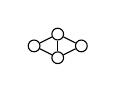
\begin{tikzpicture}[myv/.style={circle, draw, inner sep=1.5pt}]
    \node (o) at (0,0) {};
    \node[myv] (v1) at (0,0.15) {};
    \node[myv] (v2) at (0,-0.15) {};
    \node[myv] (v3) at (-0.3,0) {};
    \node[myv] (v4) at (0.3,0) {};

    \draw (v1) -- (v2);
    \draw (v1) -- (v3);
    \draw (v1) -- (v4);
    \draw (v2) -- (v3);
    \draw (v2) -- (v4);

\end{tikzpicture}, and 
a star graph on $t+1$ vertices, denoted by $K_{1,t}$,
is the tree with $t$ degree-1 vertices and one degree-$t$ vertex. The degree-$t$ vertex of a star is known as the center of the star.
 For example, $K_{1,3}$, also known as a claw,
is the graph 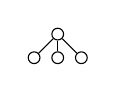
\begin{tikzpicture}[myv/.style={circle, draw, inner sep=1.5pt}]
    \node[myv] (o) at (0,0) {};
    \node[myv] (v1) at (-0.3,-0.3) {};
    \node[myv] (v2) at (0,-0.3) {};
    \node[myv] (v3) at (0.3,-0.3) {};
    \draw (o) -- (v1);
    \draw (o) -- (v2);
    \draw (o) -- (v3);
\end{tikzpicture}
. A complete graph
on $t$ vertices is denoted by $K_t$. By $\overline{G}$ we denote the complement graph of $G$. The open neighborhood and closed neighborhood of a vertex $v$ are denoted by $N(v)$
and $N[v]$ respectively. The underlying graph will be evident from the context. 
For a subset $S$ of vertices of $G$, by $G[S]$ we 
denote the graph induced by $S$ in $G$.
For a given graph $G$ and a set  $S\subseteq V(G)$, we define the graph
$G\oplus S$ as the graph obtained from $G$ by complementing the subgraph induced by $S$, i.e., 
an edge $uv$ is in $G\oplus S$ if and only if 
$uv$ is a nonedge in $G$ and $u,v\in S$, or $uv$ is 
an edge in $G$ and $\{u,v\} \setminus S \neq \emptyset$.
The operation is called subgraph complementation.
Let $\mathcal{H}$ be a set of graphs. We say that a graph $G$ is $\mathcal{H}$-free if $G$ does not have any induced copies of any of the graphs in $\mathcal{H}$. If $\mathcal{H}=\{H\}$, then we say that $G$ is $H$-free. The general definition of the problem that we deal with is given below. 
\begin{mdframed}
  \textbf{\SCT{$\mathcal{G}$}\ }:  
  Given a graph $G$,  find whether there is a set $S\subseteq V(G)$ such that $G\oplus S \in \mathcal{G}$ .
\end{mdframed}

In a parameterized problem, apart from the usual input, there is an additional integer input known as the parameter. A graph problem is fixed-parameter tractable (FPT)
if it can be solved in time $f(k)n^{O(1)}$, where $n$
is the number of vertices and $f(k)$ is any computable function. A parameterized problem admits a kernel if there is a polynomial-time algorithm which takes as input an instance $(I',k')$ of the problem and outputs
an instance $(I,k)$ of the same problem so that
$|I|,k\leq f(k)$ for some computable function $f(k)$, and
$(I',k')$ is a yes-instance if and only if $(I,k)$
is a yes-instance (here, $k'$ and $k$ are the parameters). A kernel is a polynomial kernel
if $f(k)$ is a polynomial function. It is known that
a problem admits an FPT algorithm if and only if it 
admits a kernel. An FPT algorithm implies that there 
is a polynomial-time algorithm to solve the problem
when the parameter is a constant. We refer to the book~\cite{DBLP:books/sp/CyganFKLMPPS15} for further exposition on these topics.



